\documentclass[xcolor=svgnames]{beamer}
\usetheme[
    %%% options passed to the outer theme
    %    hidetitle,           % hide the (short) title in the sidebar
    %    hideauthor,          % hide the (short) author in the sidebar
    %    hideinstitute,       % hide the (short) institute in the bottom of the sidebar
    %    shownavsym,          % show the navigation symbols
         width=1.5cm,         % width of the sidebar (default is 2 cm)
    %    hideothersubsections,% hide all subsections but the subsections in the current section
    %    hideallsubsections,  % hide all subsections
         left                 % right of left position of sidebar (default is right)
    %%% options passed to the color theme
        lightheaderbg         % use a light header background
  ]{AAUsidebar}
\setbeameroption{show notes}

% #### graphics and schemes
\usepackage{graphicx}
\graphicspath{{img/}}
\usepackage{tikz}
\usetikzlibrary{                          % TikZ libraries
                scopes,                   % .
                shapes,                   % .
                arrows,                   % .
                through,                  % .
                calc,                     % .
                intersections,            % .
                spy,                      % .
                matrix,                   % .
                chains,                   % .
                mindmap,                  % .
                trees,                    % .
                decorations.pathreplacing,% .
                decorations.pathmorphing, % .
                decorations.markings}     % .

\usepackage{pgfplots}                     % TikZ plots
\usepackage{pgfplotstable}                % TikZ tables from CSV
\pgfplotsset{compat=1.3}                  % activates \xilabel shift` for pgfplots
\usepackage{array}
\usepackage{listings}
\usepackage{times}
\usepackage{amsmath}
\usepackage{verbatim}
\usepackage{ccicons}
\usepackage{tcolorbox}
\usepackage{chronosys}
\usepackage{listings}                     % code
\usepackage{adjustbox}                    % code
\usepackage{attrib}

% #### colors
\usepackage{xcolor}                       % common color names
\usepackage{colortbl}                     % common color names

% #### layouts
\usepackage{multicol}
\usepackage[textfont=footnotesize,bf]{caption}
\usepackage{subfig}

% #### fonts
\usepackage[utf8]{inputenc}
\usepackage[english]{babel}
\usepackage[T1]{fontenc}
\usepackage{cmbright}
\usepackage{soul} %slanted text
\usepackage{hyperref}
\urlstyle{same}
\hypersetup{pdfauthor={Francesco de Virgilio},pdftitle={HIRMEOS WP 5 / 6: London validation workshop}}

% #### tables
\usepackage{booktabs}			          % migliora la qualità delle tabelle
\usepackage{tabularx}			          % colonne a spaziatura fissa delle tabelle
\newcommand{\otoprule}                    % better top rule horizontal line
    {\midrule[\heavyrulewidth]}           % .


\begin{document}

\usebackgroundtemplate{
    
\includegraphics[width=\paperwidth,height=\paperheight]{img/cover}
}

    \begin{frame}[plain,noframenumbering]
        \begin{center}
            \color{RoyalBlue}
            \textbf{
                \Huge{HIRMEOS WP 5 / 6}\\
                \Large{London validation workshop}\\
            }
            \vspace{40pt}
            Francesco de Virgilio\\
            \vspace{8pt}
            \scriptsize{Tech Team Lead, Ubiquity Press}\\
            \scriptsize{London, 19/06/2018}
        \end{center}
    \end{frame}

\usebackgroundtemplate{%
    
\includegraphics[width=\paperwidth,height=\paperheight]{img/background}
}

\section{WP 5: annotations}

    \subsection{Libraries}

        \begin{frame}{Objectives}
            annotations of different formats: HTML, ePub, PDF
            identified usable versions of libraries:
            \begin{itemize}
                \item hypothes.is --- 1.84.0
                \item epub.js --- 0.3.63
                \item pdf.js --- 1.1.114
            \end{itemize}
            \pause
            \begin{block}{Ubiquity's HIRMEOS CDN}
                Based on Google Cloud CDN: \texttt{https://storage.googleapis.com/hirmeos/}
            \end{block}
        \end{frame}

    \subsection{Aggregation}

        \begin{frame}{Objectives}
            \begin{block}{automatic resolution of identifiers (figures, chapters) to book}
                implementation in WP6
            \end{block}
            \begin{block}{aggregation of metrics}
                implementation in WP6
            \end{block}
        \end{frame}

    \subsection{Documentation}

        \begin{frame}{Objectives}
            documentation
            \begin{block}{usage, development}
                \texttt{docs.metrics.ubiquity.press}
            \end{block}
            \begin{block}{API docs}
                \texttt{metrics.ubiquity.press/api/docs}
            \end{block}
        \end{frame}

    \subsection{Code}

        \begin{frame}{Objectives}
            open source code
            \begin{block}{on GitHub}
                \texttt{https://github.com/hirmeos/metrics}
            \end{block}
        \end{frame}

    \subsection{How it works}

        \begin{frame}{How it works}
            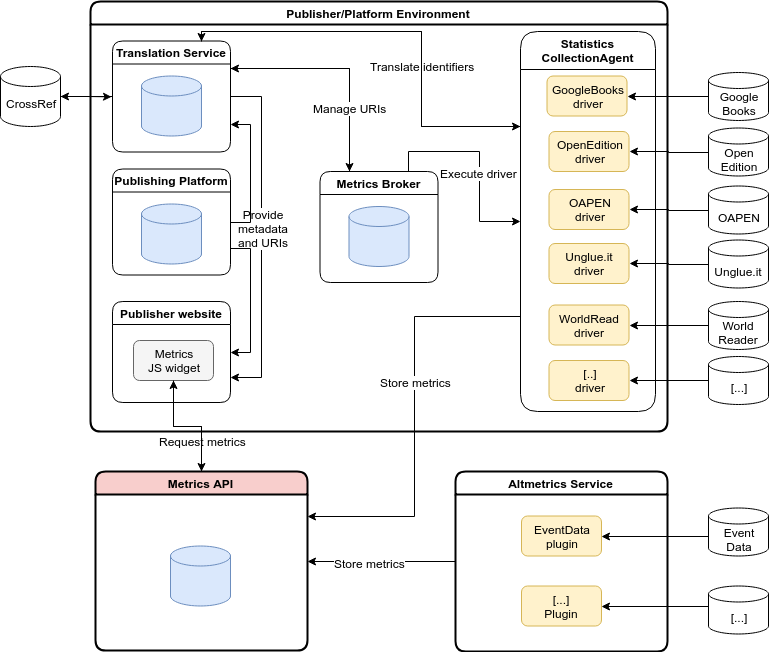
\includegraphics[width=0.8\textwidth]{img/metrics-servicehirmeos-wp6.png}
        \end{frame}

\section{WP 6: altmetrics}

    \begin{frame}{Plugins}
        \begin{itemize}
            \item annotations --- completed
            \item CrossRef cited by --- almost completed
            \item wikipedia --- WIP
            \item twitter, by DOI --- todo
            \item twitter, by URL --- todo
            \item facebook, by DOI --- todo
            \item facebook, by URL --- todo
        \end{itemize}
    \end{frame}

    \begin{frame}{Scalability}
        \begin{itemize}
            \item RabbitMq
            \item Celery (Django)
            \item periodically, a new task is creataed for each source, for eache DOI
            \item tasks are consumed by a flexible amount of workers (automatic scaling)
        \end{itemize}
    \end{frame}

    \begin{frame}{Edits}
        \begin{itemize}
            \item added API endpoint to POST DOIs and URLs
            \item testing Wordpress.com as source (more to come?)
            \item setup integration testing (\texttt{https://ci.ubiquity.press/\#/builders/9})
        \end{itemize}
    \end{frame}

    \begin{frame}{Thanks}
        \begin{center}
            \Huge{www.hirmeos.eu}
        \end{center}
        \vspace{0.5\textheight}
        \begin{center}
            \Large{francesco.devirgilio@ubiquitypress.com}
        \end{center}
    \end{frame}

\end{document}
